%! TEX root = ../main.tex
\documentclass[main]{subfiles}

\begin{document}
\chapter{提案システム}
本章では,本研究で提案するグロシシステムについて説明する.

\section{用語の定義}
本節では,以下本論文で使用する用語を定義する.

\begin{definition}あたらしい用語\\
あたらしい用語とは,この論文の中で使用される,一般的ではない語句のことである.
\end{definition}

\begin{definition}グロシ\\
    グロシってなんだよへへっ.ぴえんぴえん.グロシって書いてあったらグロシって読むしかないだろう?
\end{definition}

\section{システムの概要}
本研究では,グロシステムを提案する.提案システムの概要を図\ref{fig:system_gaiyou_1}に示す.

% 図の例
\begin{figure}[htb]
    \centering
    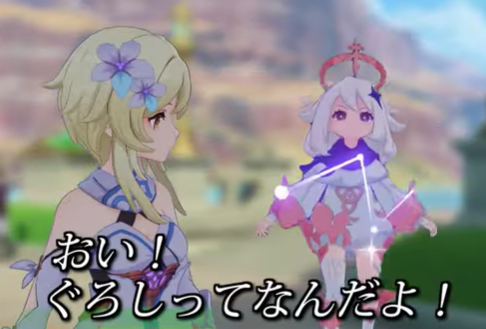
\includegraphics[width=0.9\linewidth]{figures/system_gaiyou_1.png}
    \caption{提案システム概要}
    \label{fig:system_gaiyou_1}
\end{figure}

システムシステム.チェックワンツー.

こちらがみっちょル2さんの,ぐろし(独唱)です.うっひょ〜〜〜~~~!視聴時ヌヴィレットさんが水神(笑)にパワハラされていたのを見て,大きな声を出したら執律庭の皆さんからの誠意で水神(笑)の人力ボイスをサービスしてもらいました.

俺の高評価次第でこの動画伸ばす事だってできるんだってことで,視聴しま〜〜〜~~~す!まずはグロシから,コラ〜!これでもかってくらい美しいグロシの中には,よくとれた音程が入っており,驚きのあまり高評価を15回押してしまいました〜!

すっかり水神(笑)も立場を弁え誠意の歓迎を貰ったところで,お次に圧倒的存在感のサビを
視聴する〜!頃すぞ〜!暴力的な死刑の中には、頃すという単語が入っており,さすがのPAIMONもチャンネルページに入って行ってしまいました〜!

ちなみに、ヌヴィレットが憂さ晴らしに公子を倒す様子はぜひ魔神任務をご覧ください.
\end{document}